\section{Example}  \label{sec:abstraction:results}

This section shows generalization on the defeatured ``Encloser'' model. It has Sheet metal features such as Face, Flange, Lofted Flange etc.


%%\bigskip

%\begin{table}[!htb]
\begin{center}
\captionof{table}{Generalizing ``Enclosure'' Model}
\begin{longtable}[h]{@{}p{0.6\linewidth} p{0.25\linewidth}@{}}
\toprule

%\begin{longtable}[h]{@{} p{0.1\linewidth}  p{0.38\linewidth} p{0.15\linewidth} p{0.2\linewidth}@{}}
%\toprule
Model & Feature Tree \\
 \midrule

\raisebox{-0.8\height}{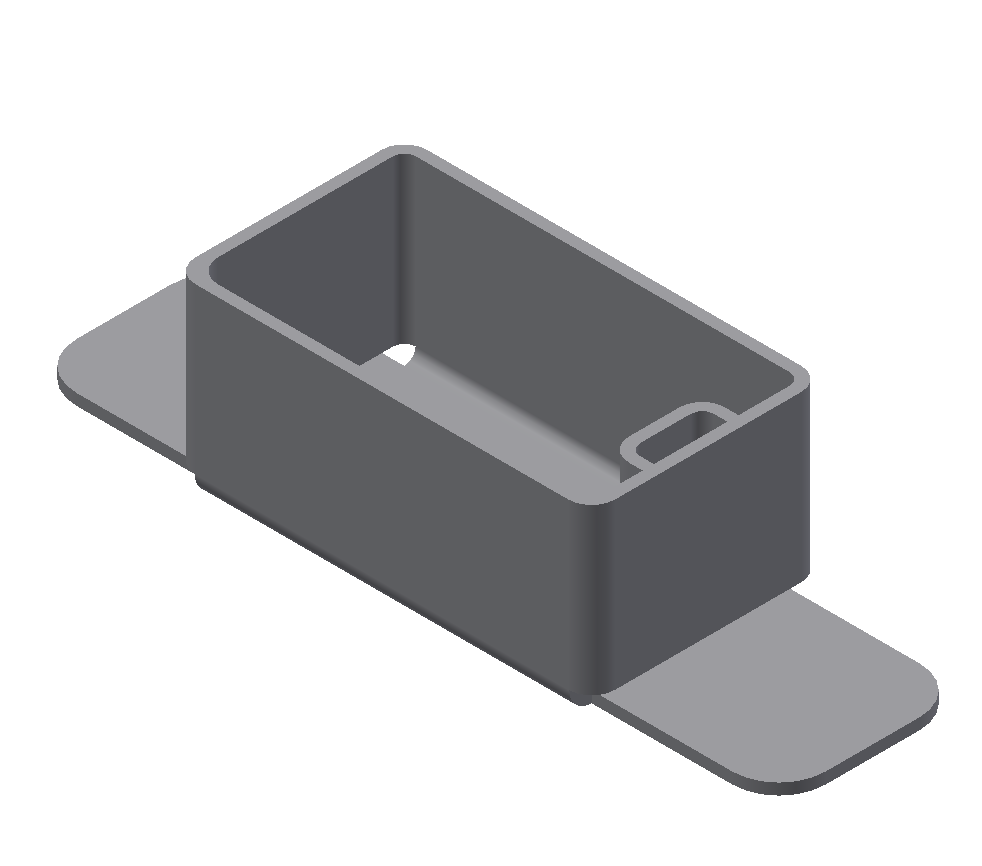
\includegraphics[width=0.9\linewidth]{images/SheetMetal_Medium_Enclosure_pre_abel_part}}  &
\raisebox{-0.8\height}{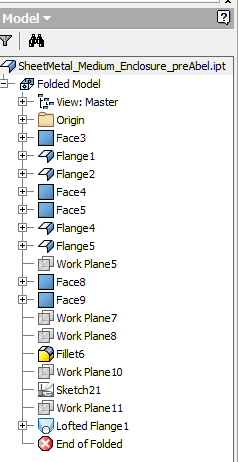
\includegraphics[width=0.9\linewidth]{images/SheetMetal_Medium_Enclosure_pre_abel_tree}} \\ \midrule

\raisebox{-0.8\height}{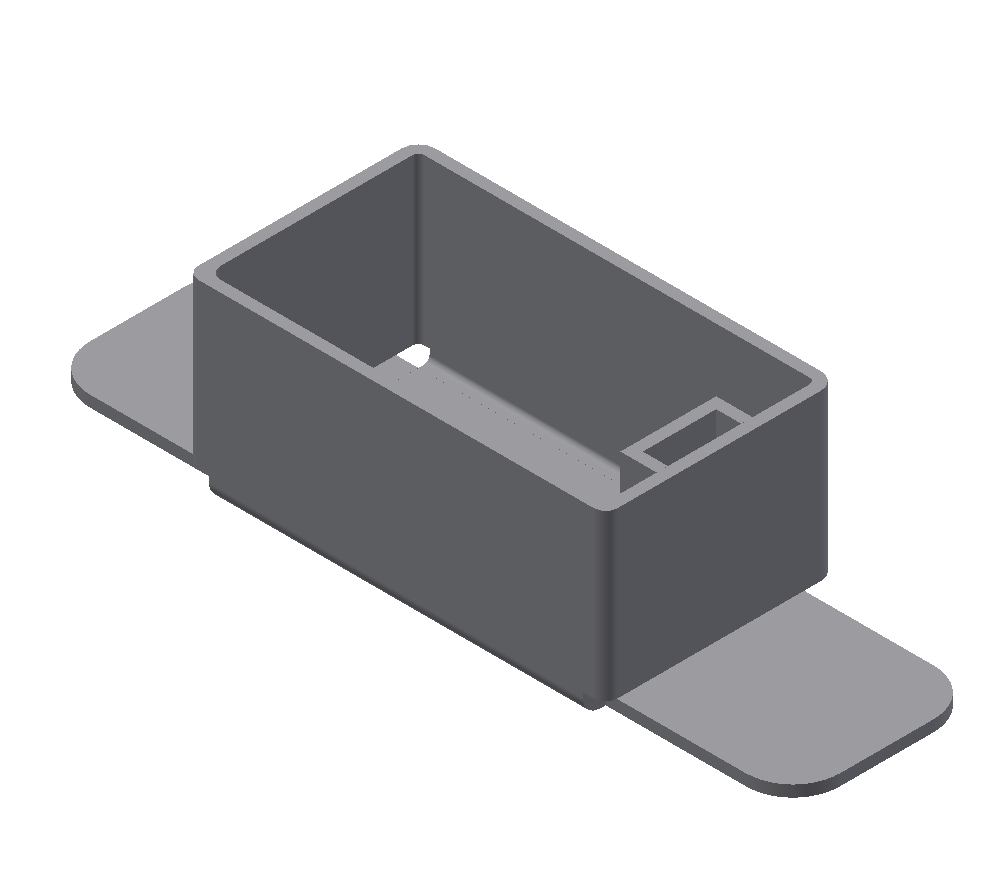
\includegraphics[width=0.9\linewidth]{images/SheetMetal_Medium_Enclosure_abel_part}} &
\raisebox{-0.8\height}{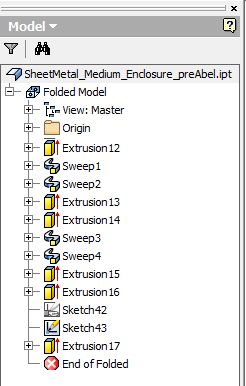
\includegraphics[width=0.9\linewidth]{images/SheetMetal_Medium_Enclosure_abel_tree}} \\

\bottomrule
\end{longtable}

\label{tbl:abstraction:enclosure}
%\end{table}
\end{center}

%%\bigskip

Table \ref{tbl:abstraction:enclosure} shows transformation of sheet metal features CAD model into $\mathcal{ABLE}$ model having only Loft-equivalent features. This result demonstrates the effectiveness of generalization module as the input model is faithfully transformed into generalized features without any feature or shape loss.
